\documentclass[]{article}
\usepackage{lmodern}
\usepackage{amssymb,amsmath}
\usepackage{ifxetex,ifluatex}
\usepackage{fixltx2e} % provides \textsubscript
\ifnum 0\ifxetex 1\fi\ifluatex 1\fi=0 % if pdftex
  \usepackage[T1]{fontenc}
  \usepackage[utf8]{inputenc}
\else % if luatex or xelatex
  \ifxetex
    \usepackage{mathspec}
    \usepackage{xltxtra,xunicode}
  \else
    \usepackage{fontspec}
  \fi
  \defaultfontfeatures{Mapping=tex-text,Scale=MatchLowercase}
  \newcommand{\euro}{€}
\fi
% use upquote if available, for straight quotes in verbatim environments
\IfFileExists{upquote.sty}{\usepackage{upquote}}{}
% use microtype if available
\IfFileExists{microtype.sty}{%
\usepackage{microtype}
\UseMicrotypeSet[protrusion]{basicmath} % disable protrusion for tt fonts
}{}
\usepackage[margin=1in]{geometry}
\usepackage{longtable,booktabs}
\usepackage{graphicx}
\makeatletter
\def\maxwidth{\ifdim\Gin@nat@width>\linewidth\linewidth\else\Gin@nat@width\fi}
\def\maxheight{\ifdim\Gin@nat@height>\textheight\textheight\else\Gin@nat@height\fi}
\makeatother
% Scale images if necessary, so that they will not overflow the page
% margins by default, and it is still possible to overwrite the defaults
% using explicit options in \includegraphics[width, height, ...]{}
\setkeys{Gin}{width=\maxwidth,height=\maxheight,keepaspectratio}
\ifxetex
  \usepackage[setpagesize=false, % page size defined by xetex
              unicode=false, % unicode breaks when used with xetex
              xetex]{hyperref}
\else
  \usepackage[unicode=true]{hyperref}
\fi
\hypersetup{breaklinks=true,
            bookmarks=true,
            pdfauthor={RESURAL (JcB)},
            pdftitle={Activité des structures d'urgences : panorama 2014 de la région ALSACE},
            colorlinks=true,
            citecolor=blue,
            urlcolor=blue,
            linkcolor=magenta,
            pdfborder={0 0 0}}
\urlstyle{same}  % don't use monospace font for urls
\setlength{\parindent}{0pt}
\setlength{\parskip}{6pt plus 2pt minus 1pt}
\setlength{\emergencystretch}{3em}  % prevent overfull lines
\setcounter{secnumdepth}{5}

%%% Use protect on footnotes to avoid problems with footnotes in titles
\let\rmarkdownfootnote\footnote%
\def\footnote{\protect\rmarkdownfootnote}

%%% Change title format to be more compact
\usepackage{titling}

% Create subtitle command for use in maketitle
\newcommand{\subtitle}[1]{
  \posttitle{
    \begin{center}\large#1\end{center}
    }
}

\setlength{\droptitle}{-2em}
  \title{Activité des structures d'urgences : panorama 2014 de la région ALSACE}
  \pretitle{\vspace{\droptitle}\centering\huge}
  \posttitle{\par}
  \author{RESURAL (JcB)}
  \preauthor{\centering\large\emph}
  \postauthor{\par}
  \predate{\centering\large\emph}
  \postdate{\par}
  \date{28/01/2015}



\begin{document}

\maketitle


{
\hypersetup{linkcolor=black}
\setcounter{tocdepth}{2}
\tableofcontents
}
Version mse à jour le: \textbf{Fri Jul 31 16:24:29 2015}

Ajout de la dernière version de Gilles

\begin{itemize}
\itemsep1pt\parskip0pt\parsep0pt
\item
  nombre de passages pour 10.000 hab.
\item
  nombre de SU pour 10.000 hab.
\item
  nombre de lignes SMUR financées par une MIG
\item
  nombre de siège de SMUR dont SMUR saisonnier dont antenne SMUR dont
  hélismur
\item
  séparer privés lucratifs et ESPIC
\item
  nombre de logicels et nombre de SU par région
\item
  SAE 2014 ?
\item
  augmentation par rapport année N-1 en tenant compte uniquement des
  établissements ``stables''
\item
  séparer chu et non chu, samu de chu et de non chu
\item
  retour attendu pour le 4/9
\end{itemize}

\section{Activité des structures d'urgences : panorama 2014 de la région
ALSACE}\label{activite-des-structures-durgences-panorama-2014-de-la-region-alsace}

Rapport 2014 respectant les préconisations de la FEDORU. Source:
\href{https://docs.google.com/document/d/101LYVqVLeHZnrujfMm3aqBYfbOwx3CPEB3Y-Lbud2Ls/edit}{Trame
commune}

Le document de référence pour le rapport est: \textbf{V4 trame commune
2014 rapport inter région} (xps:
/home/jcb/Documents/Resural/FEDORU/Trame\_Commune/DOC/Trame commune 2014
rapport inter région (V4).docx)

\textbf{NOTE}: certaines informations utiles sont dans
\textbf{RPU\_Doc}.

\section{LE MOT DU PRÉSIDENT DE LA
FEDORU}\label{le-mot-du-president-de-la-fedoru}

La publication du panorama des urgences de la région
\textbf{ALSACE}constitue une excellente occasion pour présenter la
fédération des observatoires régionaux des urgences (FEDORU) qui compte
\textbf{RESURAL} parmi ses membres actifs.

La FEDORU a été créée au mois d'octobre 2013. Ses membres sont chargés
dans leur région respective du traitement des données d'urgences ; ce
point commun est le trait d'origine de la FEDORU et donne son empreinte
à l'objet de notre association que je cite ici :

\begin{itemize}
\itemsep1pt\parskip0pt\parsep0pt
\item
  promouvoir les observatoires régionaux des urgences et les structures
  ayant une activité similaire ;
\item
  promouvoir toutes les actions visant à améliorer la connaissance sur
  les soins de premier recours ;
\item
  partager les expertises dans le domaine du recueil, de l'analyse et de
  l'évaluation de la qualité des données relatives à l'activité des
  urgences.
\end{itemize}

Les premières publications de la FEDORU (disponibles sur le site :
\url{http://www.fedoru.fr}) abordent les thèmes techniques suivants :

\begin{itemize}
\itemsep1pt\parskip0pt\parsep0pt
\item
  Recommandations pour la création d'un ORU
\item
  Collecte et usage des RPU
\item
  Hôpital en tension - Synthèse FEDORU
\end{itemize}

Ces documents constituent le socle indispensable à la conduite de
travaux inter-régionaux. Nous pourrons ainsi comparer nos résultats,
harmoniser les indicateurs retenus dans nos publications respectives,
travailler sur des échantillons de données plus importants(inter-région
ou national), mais aussi évaluer l'impact de différentes organisations.

La recherche de consensus et d'échanges entre les différents acteurs
régionaux représentés au sein de la FEDORU s'illustre parfaitement dans
cette publication qui prend le parti de respecter les premières
recommandations sur le traitement des RPU. Le ``panorama des urgences en
région \ldots{}.'', intègre le format d'analyse commun 2015 proposé de
manière collégiale par nos groupes experts et validé par notre conseil
d'administration. Ce socle d'analyse produit par ``la structure
concernée'' sera rapproché des résultats des autres régions et donnera
lieu à une publication commune au cours de l'année 2015. J'adresse au
nom de la FEDORU toutes mes félicitations à l'ensemble de l'équipe de
\textbf{RESURAL} pour la qualité de leurs travaux mais aussi et surtout
à tous les professionnels des services d'urgences de l'\textbf{ALSACE}
pour le fastidieux mais si précieux travail de collecte sur le terrain.

\textbf{Dr G. VIUDES}

\emph{Président de la FEDORU}

\section{Description de l'offre de
soins}\label{description-de-loffre-de-soins}

\subsection{Qualité des données}\label{qualite-des-donnees}

Réalisation d'un diagramme radar présentant l'exhaustivité des items
RPU.

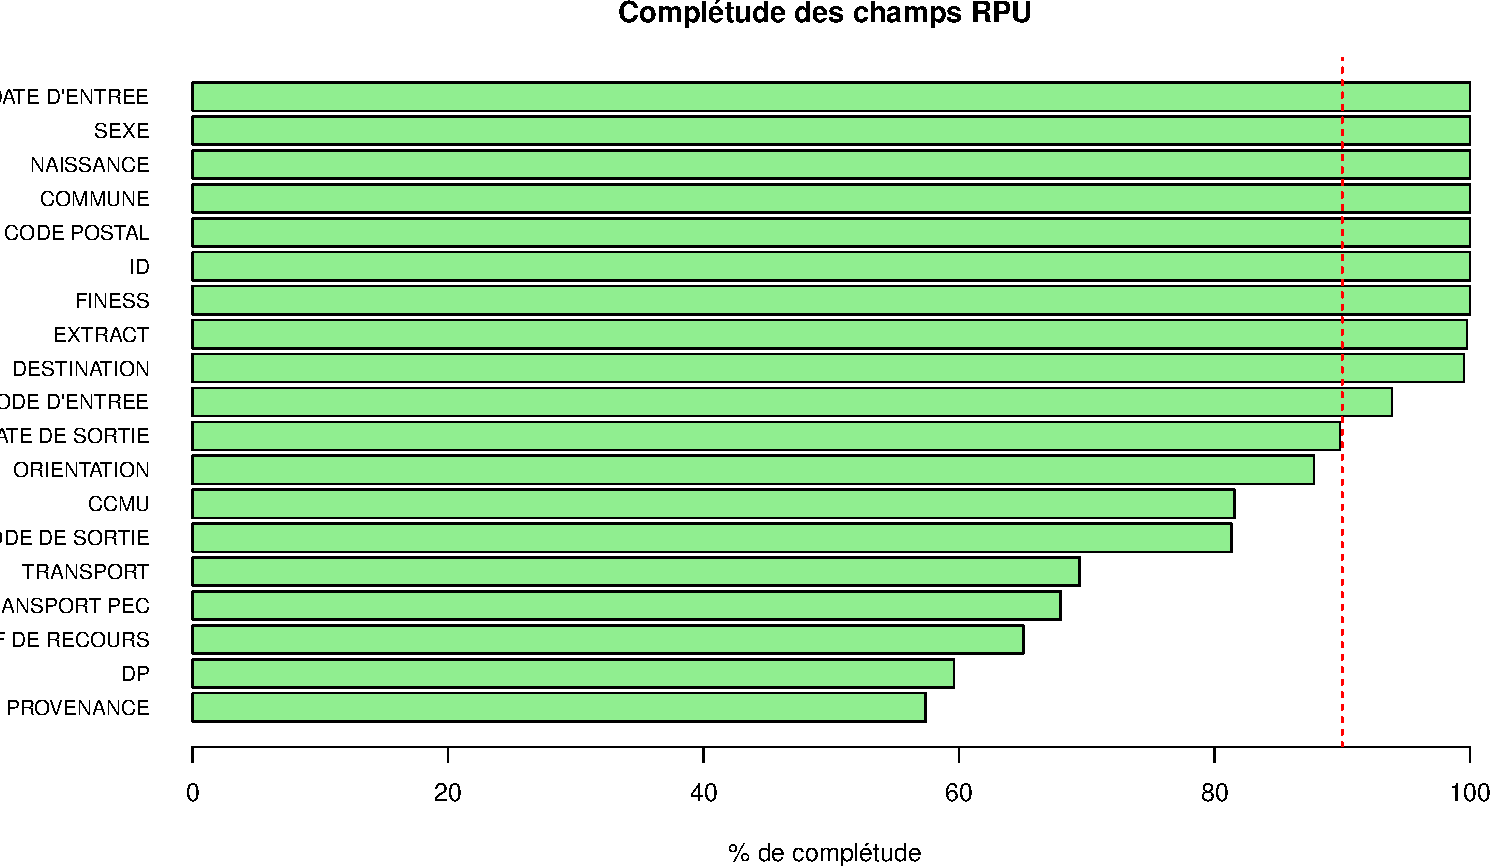
\includegraphics{rapport2014_V4_files/figure-latex/completude-1.pdf}
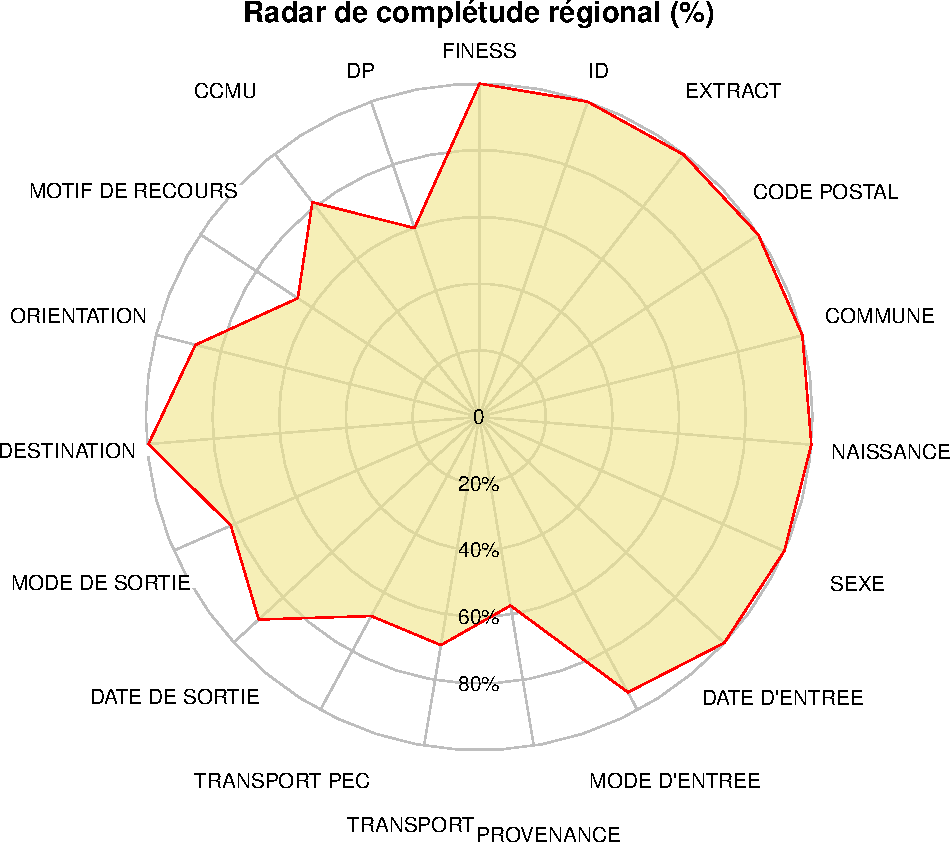
\includegraphics{rapport2014_V4_files/figure-latex/completude-2.pdf}

Complétude en valeur absolue et en pourcentages:`

\begin{verbatim}
##           FINESS               ID          EXTRACT      CODE POSTAL 
##           416733           416733           415731           416733 
##          COMMUNE        NAISSANCE             SEXE    DATE D'ENTREE 
##           416716           416733           416733           416733 
##    MODE D'ENTREE       PROVENANCE        TRANSPORT    TRANSPORT PEC 
##           391370           239122           289308           283189 
##   DATE DE SORTIE   MODE DE SORTIE      DESTINATION      ORIENTATION 
##           374349           338878            82635            72898 
## MOTIF DE RECOURS             CCMU               DP 
##           270962           339827           245974
\end{verbatim}

\begin{verbatim}
##           FINESS               ID          EXTRACT      CODE POSTAL 
##              100              100              100              100 
##          COMMUNE        NAISSANCE             SEXE    DATE D'ENTREE 
##              100              100              100              100 
##    MODE D'ENTREE       PROVENANCE        TRANSPORT    TRANSPORT PEC 
##               94               57               69               68 
##   DATE DE SORTIE   MODE DE SORTIE      DESTINATION      ORIENTATION 
##               90               81              100               88 
## MOTIF DE RECOURS             CCMU               DP 
##               65               82               60
\end{verbatim}

\section{Les chiffres clés de l'activité des services
d'urgences}\label{les-chiffres-cles-de-lactivite-des-services-durgences}

\subsection{Recueil des données}\label{recueil-des-donnees}

\begin{itemize}
\itemsep1pt\parskip0pt\parsep0pt
\item
  Nombre de passages dans l'année {[}C{]}: 416 733 RPU
\item
  Moyenne quotidienne de passages {[}C{]}: 1 142 RPU
\item
  \%(N) d'évolution par rapport à année N-1 {[}C{]}: 122 \%.
\item
  \% d'évolution moyenne sur les 5 dernières années (méthode calcul :
  moyenne des évolutions constatées entre chaque année)
\item
  Données renseignées (données à partir desquelles tout le reste de
  l'analyse sera effectuée)

  \begin{itemize}
  \itemsep1pt\parskip0pt\parsep0pt
  \item
    Nombre de RPU transmis: 416 733 RPU
  \item
    Exhaustivité du recueil : Nb RPU transmis / Nb de passages déclarés
    84 \% (NOTE le nombre de passages déclarés est celui indiqué par les
    données SAE 2013)
  \end{itemize}
\end{itemize}

\subsection{PATIENTS}\label{patients}

\subsubsection{SEXE}\label{sexe}

\begin{itemize}
\itemsep1pt\parskip0pt\parsep0pt
\item
  \%(N) Femme {[}C{]}: 47.78 \% (199 110)
\item
  \%(N) Homme {[}C{]}: 52.22 \% (217 617)
\item
  Sex ratio: 1.09
\item
  Taux de masculinité: 0.52
\end{itemize}

\subsubsection{Age}\label{age}

\begin{itemize}
\item
  age moyen{[}C{]}: 38.03 ans.
\item
  age moyen des hommes {[}S{]}: 35.93 ans.
\item
  age moyen des femmes {[}S{]}: 40.31 ans.
\item
  \% (N) \textless{} 1 an {[}C{]}: 15 376 (3.69 \%)
\item
  \%(N) \textless{} 15 ans {[}C{]}: 103 413 (24.82 \%)
\item
  \%(N) \textless{} 18 ans {[}C{]}: 119 213 (28.61 \%)
\item
  \%(N) \textgreater{}= 75 ans {[}C{]}: 57 271 (13.74 \%)
\item
  Pyramide des ages:
\end{itemize}

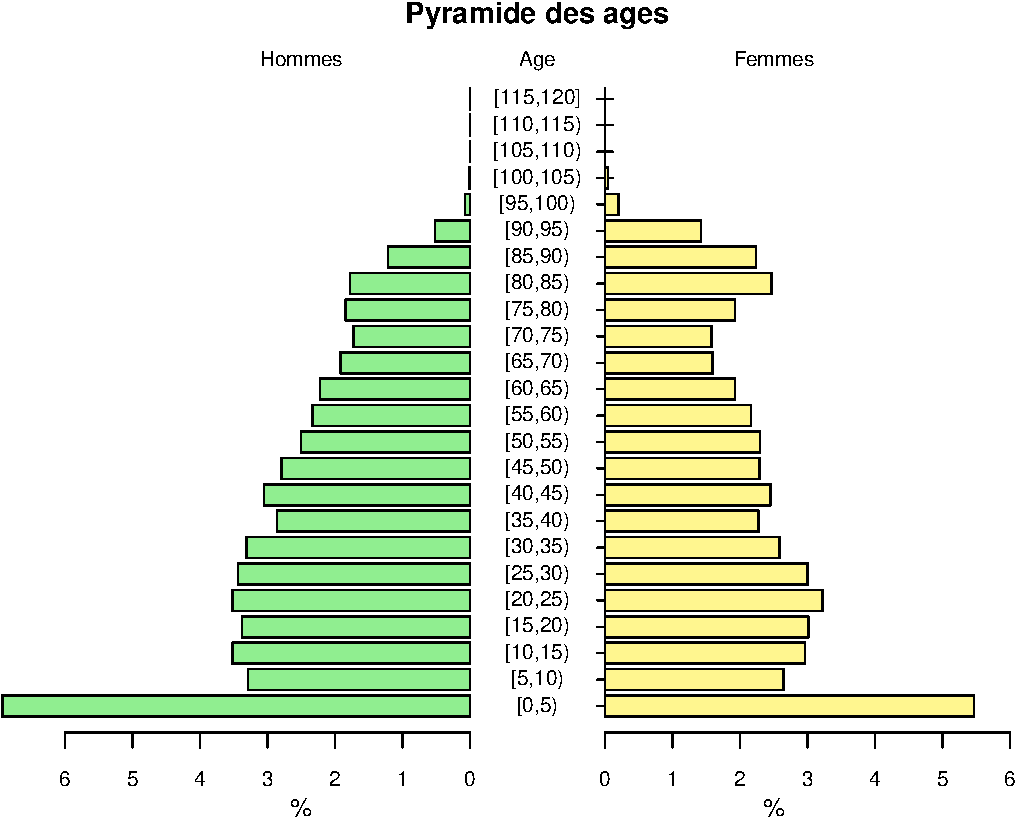
\includegraphics{rapport2014_V4_files/figure-latex/pyramide-1.pdf}

\begin{verbatim}
## [1] 5.1 4.1 4.1 2.1
\end{verbatim}

\subsubsection{Taux de recours (définition FEDORU) régional aux
urgences.
{[}S{]}}\label{taux-de-recours-definition-fedoru-regional-aux-urgences.-s}

Utilisation des données INSEE qui collent le plus à la période d'étude
(projections ou données consolidées)

TARRU: \textbf{21.31\%} (ref: population alsacienne 2014)

\subsubsection{\% de patients ne venant pas de la région (étranger
compris)}\label{de-patients-ne-venant-pas-de-la-region-etranger-compris}

4.43\%

\subsection{ARRIVÉE}\label{arrivee}

\subsubsection{Horaires de passage}\label{horaires-de-passage}

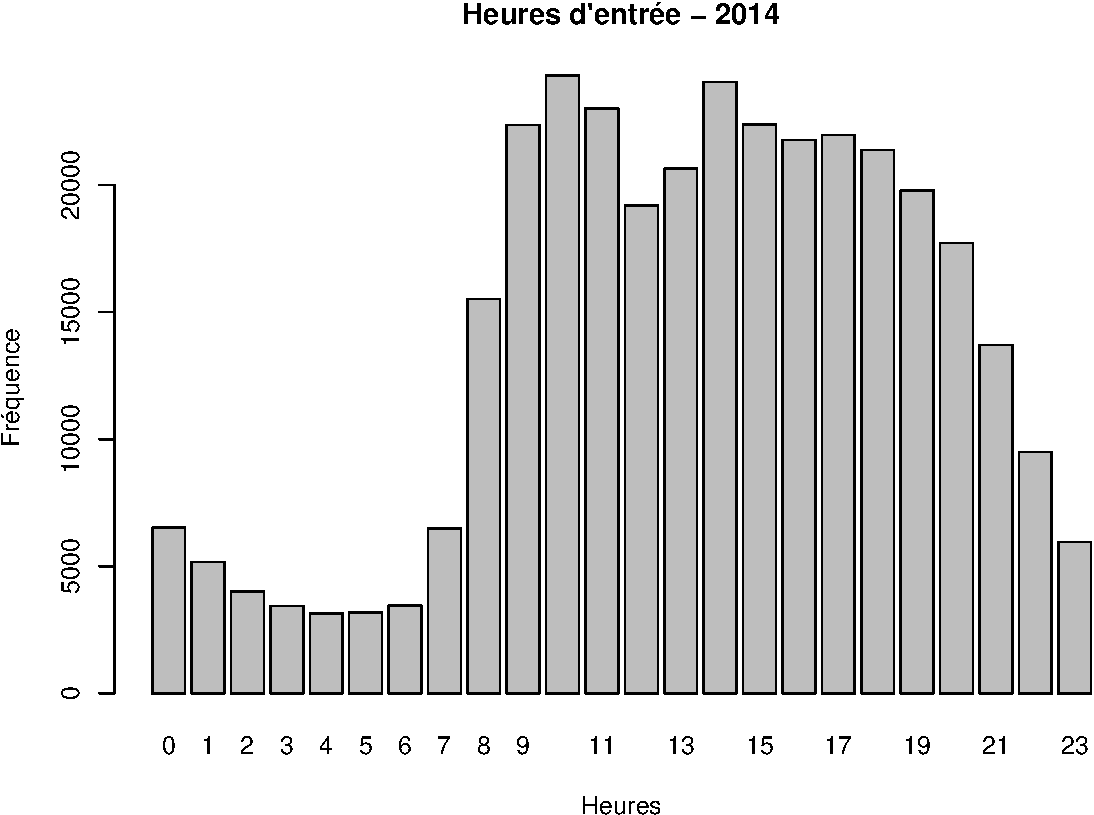
\includegraphics{rapport2014_V4_files/figure-latex/horaires-1.pdf}

\begin{itemize}
\item
  \% passages nuit {[}C{]}: 24.74 \% (N = 92 610)
\item
  \% passages nuit profonde {[}C{]}: 11.09 \% (N = 41 500)
\item
  \% passages en horaire de PDS: 45.22 \% (Remarque: ne tient pas compte
  des jours fériés survenant en semaine)
\end{itemize}

\subsubsection{Moyens d'arrivée}\label{moyens-darrivee}

\begin{itemize}
\itemsep1pt\parskip0pt\parsep0pt
\item
  \textbf{\%(N) d'arrivée personnel} {[}S{]}: 72.16 \% (N = 208 771)
\item
  \textbf{\%(N) d'arrivée SMUR} {[}S{]}: 0.93 \% (N = 2 702)
\item
  \textbf{\%(N) d'arrivée VSAB} {[}S{]}: 10.35 \% (N = 29 954)
\item
  \textbf{\%(N) d'arrivée Ambulance} {[}S{]}: 15.94 \% (N = 46 112)
\end{itemize}

NB : commentaire possible pour expliquer que la somme des 4 pourcentages
ci dessus ne fait pas 100 \%

\subsubsection{Gravité (CCMU)}\label{gravite-ccmu}

\begin{itemize}
\itemsep1pt\parskip0pt\parsep0pt
\item
  \textbf{\%(N) CCMU 1 et 2} {[}C{]}: 84.45\% (n = 286 979)
\item
  \textbf{\%(N) CCMU 4 et 5} {[}C{]}: 1.28\% (n = 4 341)
\end{itemize}

DIAGNOSTIC PRINCIPAL

Remarque: les chiffres sont dans le document
\emph{Codes}regroupement\_ORUMIP\_ =\textgreater{} à rajouter.

\begin{itemize}
\itemsep1pt\parskip0pt\parsep0pt
\item
  \% Médico-chirurgical
\item
  \% Traumatologique
\item
  \% Psychiatrique
\item
  \% Toxicologique
\item
  \% Autres recours
\end{itemize}

\subsubsection{Durées de passage}\label{durees-de-passage}

\begin{itemize}
\item
  durée moyenne de passage 155 mn.
\item
  écart-type: 171.59 mn.
\item
  médiane: 109 mn.
\item
  nombre de passages \textgreater{} 4 heures: 69 521 (18.69 \%).
\item
  nombre de passages inférieurs ou égaux à 4 heures: 302 546 (81.31 \%).
\item
  Lors d'une hospitalisation post-urgences (hospitalisation = mutation +
  transfert)

  \begin{itemize}
  \itemsep1pt\parskip0pt\parsep0pt
  \item
    médiane durée de passage en cas de retour à domicile: \textbf{104
    minutes}.
  \item
    médiane durée de passage en cas d'hospitalisation: \textbf{148
    minutes}.
  \end{itemize}
\item
  Lors d'un retour au domicile

  \begin{itemize}
  \itemsep1pt\parskip0pt\parsep0pt
  \item
    moyenne durée de passage en cas de retour à domicile: \textbf{145.87
    minutes}.
  \item
    moyenne durée de passage en cas d'hospitalisation: \textbf{187.55
    minutes}.
  \end{itemize}
\end{itemize}

(source: temps de passages.Rmd)

\subsubsection{MODE DE SORTIE}\label{mode-de-sortie}

\begin{itemize}
\itemsep1pt\parskip0pt\parsep0pt
\item
  \% (N) de retour à domicile: 75.5 \% (N = 255 852)
\item
  \% (N) Hospitalisation: 24.5 \% (N = 83 024)
\item
  \% (N) Mutation: 22.72 \% (N = 76 999)
\item
  \% (N) Transfert: 1.78 \% (N = 6 025)
\end{itemize}

\section{Les chiffres clés de l'activité des
SAMU}\label{les-chiffres-cles-de-lactivite-des-samu}

(à partir des données SRVA ``officielles'')

\begin{itemize}
\itemsep1pt\parskip0pt\parsep0pt
\item
  Nombre de dossiers de régulation médicale (DRM): 480303
\item
  Nombre de SMUR : 25 321

  \begin{itemize}
  \itemsep1pt\parskip0pt\parsep0pt
  \item
    dont primaires: format.n(19714)
  \end{itemize}
\item
  Nombre d'ambulances privées à la demande du SAMU: format.n(46031)
\end{itemize}

\section{Les chiffres clés de l'activité pédiatrique des services
d'urgences (moins de 18
ans)}\label{les-chiffres-cles-de-lactivite-pediatrique-des-services-durgences-moins-de-18-ans}

\begin{verbatim}
## ped
##      <28j  28j-1an[   1-5ans[  5-10ans[ 10-15ans[ 15-18ans[ 
##      1791     13554     36287     24738     27012     15800
\end{verbatim}

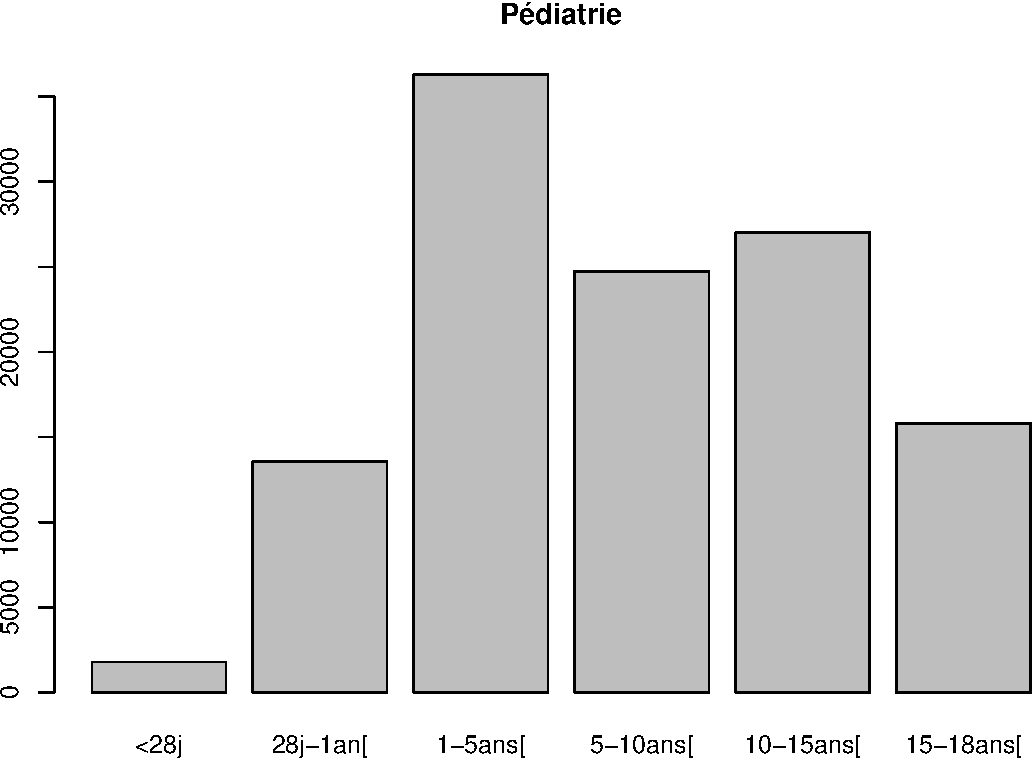
\includegraphics{rapport2014_V4_files/figure-latex/pop18-1.pdf}

\subsection{RECUEIL DES DONNÉES}\label{recueil-des-donnees-1}

\begin{itemize}
\itemsep1pt\parskip0pt\parsep0pt
\item
  Nombre de passages dans l'année: 119 213
\item
  Moyenne quotidienne de passage: 327 passages/j
\item
  Taux d'urgences pédiatriques {[}(Nb RPU Pédia/ Nb RPU global)x100{]}:
  29 \%
\item
  TODO: \% d'évolution par rapport à l'année N-1(données SAE pour ceux
  qui n'ont pas d'historique RPU fiable et permettant la comparaison,
  préciser l'origine des données)
\end{itemize}

\subsection{PATIENTS}\label{patients-1}

\begin{itemize}
\itemsep1pt\parskip0pt\parsep0pt
\item
  Sex ratio: 1.22
\item
  Pyramide des âges (âge par année, borne supérieure toujours exclue)
\item
  Par sous classes d'âge:
\end{itemize}

\section{Les chiffres clés de l'activité gériatrique des services
d'urgences (plus de 75
ans)}\label{les-chiffres-cles-de-lactivite-geriatrique-des-services-durgences-plus-de-75-ans}

\subsection{RECUEIL DES DONNÉES}\label{recueil-des-donnees-2}

\begin{itemize}
\itemsep1pt\parskip0pt\parsep0pt
\item
  Nombre de passages dans l'année: 54 310
\item
  Moyenne quotidienne de passage: 149 passages/j
\item
  Taux d'urgences gériatriques {[}(Nb RPU Géria/ Nb RPU global)x100{]}:
  13.03 \%
\item
  TODO: \% d'évolution par rapport à l'année N-1(données SAE pour ceux
  qui n'ont pas d'historique RPU fiable et permettant la comparaison,
  préciser l'origine des données)
\end{itemize}

\subsection{PATIENTS}\label{patients-2}

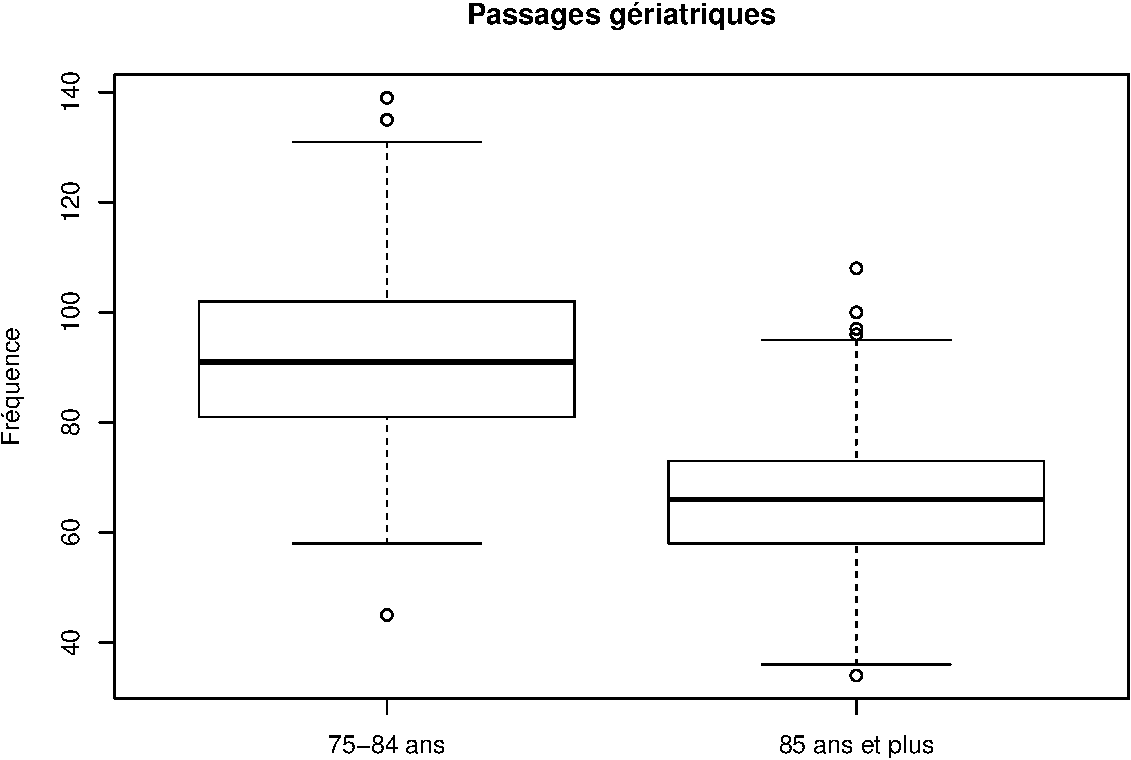
\includegraphics{rapport2014_V4_files/figure-latex/sexe75-1.pdf}

\begin{verbatim}
               effectif moyenne par jour  médiane par jour sex ratio
75-84 ans         30438                83               83      0.80
85 ans et plus    23872                65               66      0.47
\end{verbatim}

\begin{itemize}
\item
  Sex ratio: 0.64
\item
  Pyramide des âges (âge par année, borne supérieure toujours exclue)
\item
  Par sous classes d'âge:

  \begin{longtable}[c]{@{}rlllc@{}}
  \toprule\addlinespace
  eff & ectif moy & enne par jour méd & iane par jour sex & ratio
  \\\addlinespace
  \midrule\endhead
  75-84 ans & 30438 & 83 & 83 & 0.80
  \\\addlinespace
  85 ans et plus & 23872 & 65 & 66 & 0.47
  \\\addlinespace
  \bottomrule
  \end{longtable}
\end{itemize}

\subsection{ARRIVÉE}\label{arrivee-1}

\subsubsection{Horaires de passage}\label{horaires-de-passage-1}

\begin{itemize}
\itemsep1pt\parskip0pt\parsep0pt
\item
  \% passages la nuit: 22.35 \% (N = 12 140)
\item
  \% passages en horaire de PDS: 36.75 \% (N = 19 960)
\end{itemize}

\subsubsection{Moyens de transport}\label{moyens-de-transport}

\begin{itemize}
\itemsep1pt\parskip0pt\parsep0pt
\item
  \% d'arrivées Moyen perso: 20.17 \% (N = 10 953)
\item
  \% d'arrivées SMUR: 1.2 \% (N = 654)
\item
  \% d'arrivées VSAV: 11.98 \% (N = 6 505)
\item
  \% d'arrivées ambulance privée: 37.91 \% (N = 20 587)
\item
  \% réponses manquantes:
\end{itemize}

NB : commentaire possible pour expliquer que la somme des 4 pourcentages
ci dessus ne fait pas 100 \%

\subsubsection{Gravité}\label{gravite}

\begin{itemize}
\itemsep1pt\parskip0pt\parsep0pt
\item
  \% CCMU 1: 4.27 \% (N = 2 318)
\item
  \% CCMU 4 et 5: 3.16 \% (N = 1 718)
\end{itemize}

\subsubsection{Diagnostic principal}\label{diagnostic-principal}

\begin{itemize}
\itemsep1pt\parskip0pt\parsep0pt
\item
  \% Médico-chirurgical, dont :

  \begin{itemize}
  \itemsep1pt\parskip0pt\parsep0pt
  \item
    \% cardio vasculaire
  \item
    \% neuro
  \item
    \% digestif
  \item
    \% respiratoire
  \end{itemize}
\item
  \% Traumatologique
\item
  \% Psychiatrique
\item
  \% Toxicologique
\item
  \% Autres recours
\end{itemize}

\subsubsection{DURÉE}\label{duree}

\begin{verbatim}
##        NA  Mutation Transfert  Domicile     Décès           
##        NA       219       318       216        NA        NA
\end{verbatim}

\begin{verbatim}
##        NA  Mutation Transfert  Domicile     Décès           
##        NA       200       250       176        NA        NA
\end{verbatim}

\begin{verbatim}
## 
##  Welch Two Sample t-test
## 
## data:  passages75$duree by passages75$DEVENIR
## t = -4.1, df = 38419, p-value = 0.00003634
## alternative hypothesis: true difference in means is not equal to 0
## 95 percent confidence interval:
##  -11.7  -4.2
## sample estimates:
## mean in group Domicile     mean in group Hosp 
##                    216                    224
\end{verbatim}

\begin{verbatim}
## [1] 0.000036
\end{verbatim}

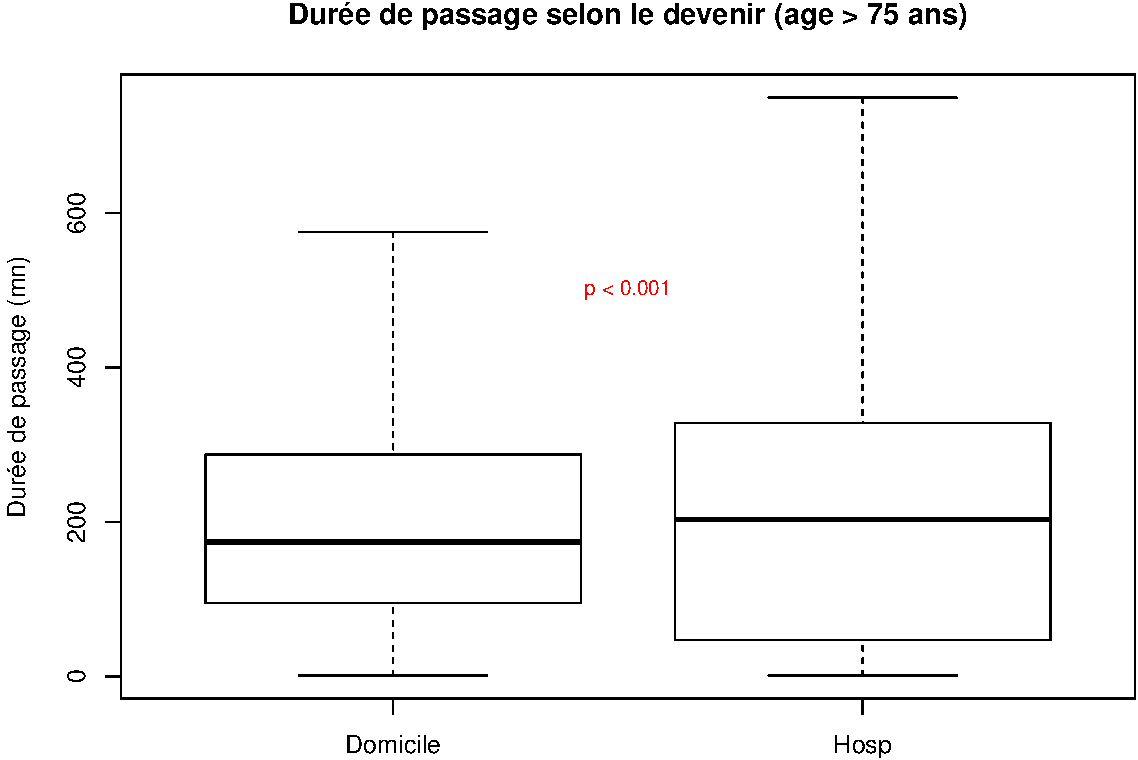
\includegraphics{rapport2014_V4_files/figure-latex/duree_passage_75-1.pdf}

\begin{itemize}
\itemsep1pt\parskip0pt\parsep0pt
\item
  Durée moyenne de passage (HORS UHCD) : 221 minutes
\item
  Durée médiane de passage (HORS UHCD) : 191 minutes
\item
  \% de passages de moins de 4h : 60.92 \%
\item
  lors d'une hospitalisation post-urgences (hospitalisation = mutation +
  transfert): 224.04 minutes.
\item
  lors d'un retour au domicile: 216.09 minutes.
\end{itemize}

\subsubsection{MODE DE SORTIE}\label{mode-de-sortie-1}

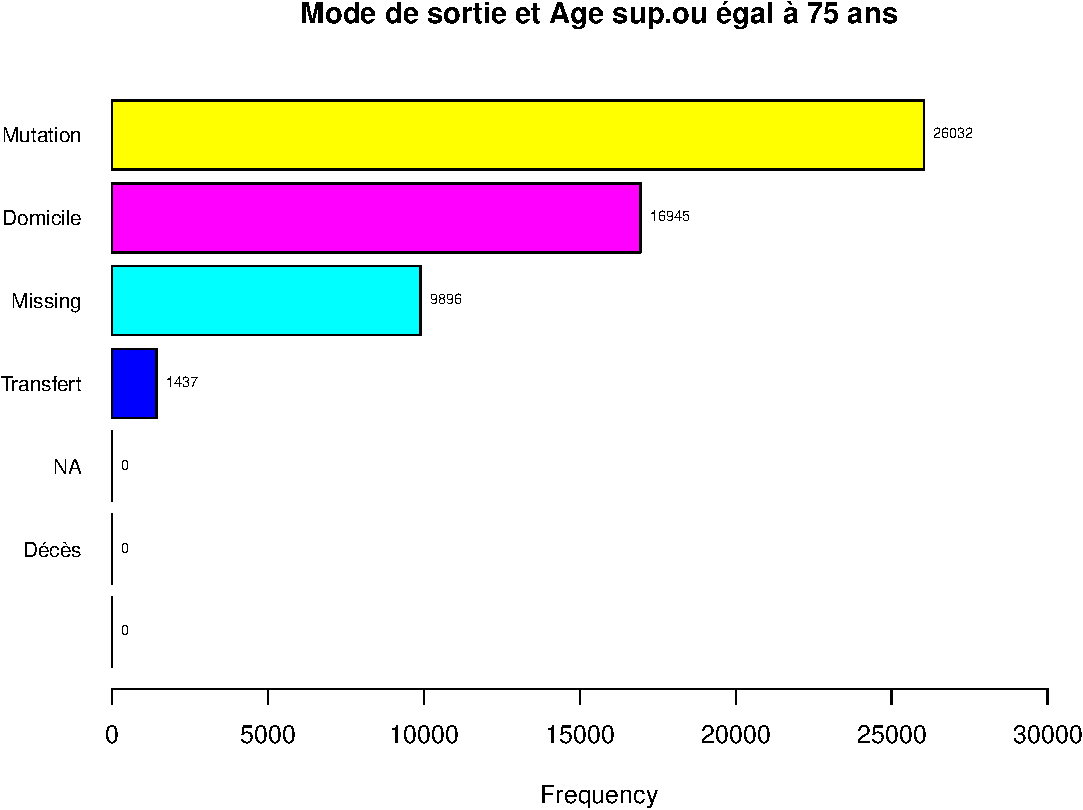
\includegraphics{rapport2014_V4_files/figure-latex/sortie75-1.pdf}

\begin{verbatim}
## pop75$MODE_SORTIE : 
##           Frequency   %(NA+)   %(NA-)
## Mutation      26032     47.9     58.6
## Domicile      16945     31.2     38.2
## NA's           9896     18.2      0.0
## Transfert      1437      2.6      3.2
## NA                0      0.0      0.0
## Décès             0      0.0      0.0
##                   0      0.0      0.0
##   Total       54310    100.0    100.0
\end{verbatim}

\begin{itemize}
\itemsep1pt\parskip0pt\parsep0pt
\item
  \% d'hospitalisation: 50.58 \% (N = 27 469)

  \begin{itemize}
  \itemsep1pt\parskip0pt\parsep0pt
  \item
    \% de mutation:47.93 \% (N = 26 032)
  \item
    \% de transfert:2.65 \% (N = 1 437)
  \end{itemize}
\item
  \% de retour à domicile:31.2 \% (N = 16 945)
\end{itemize}

\section{Les chiffres clés de l'activité AVC des services
d'urgences}\label{les-chiffres-cles-de-lactivite-avc-des-services-durgences}

\subsection{RECUEIL DES DONNÉES}\label{recueil-des-donnees-3}

\begin{itemize}
\itemsep1pt\parskip0pt\parsep0pt
\item
  Nombre d'AVC dans l'année (+ rappeler le pourcentage d'exhaustivité du
  DP par rapport au nombre de RPU): \textbf{2 949}
\item
  Moyenne quotidienne d'AVC: \textbf{8,1 AVC/j}
\item
  \% d'AVC dans l'activité globale: \textbf{1.19 \%}
\end{itemize}

\subsection{PATIENTS}\label{patients-3}

\begin{verbatim}
## c.age
##     [0,5)    [5,10)   [10,15)   [15,20)   [20,25)   [25,30)   [30,35) 
##        10         2         4        10        19        26        26 
##   [35,40)   [40,45)   [45,50)   [50,55)   [55,60)   [60,65)   [65,70) 
##        33        68        97       150       166       235       284 
##   [70,75)   [75,80)   [80,85)   [85,90)   [90,95)  [95,100) [100,105) 
##       295       393       496       408       193        28         4 
## [105,110) [110,115) [115,120) 
##         1         1         0
\end{verbatim}

\includegraphics{rapport2014_V4_files/figure-latex/patients-1.pdf}

\begin{itemize}
\itemsep1pt\parskip0pt\parsep0pt
\item
  Sex ratio: 0.95
\item
  Age moyen: 71.44 ans
\item
  Nombre d'AVC par sous classe d'âge (GT1):
\end{itemize}

\subsection{ARRIVÉE}\label{arrivee-2}

\begin{itemize}
\itemsep1pt\parskip0pt\parsep0pt
\item
  Nombre d'AVC et \% par tranche d'heure GT1 (matinée, début d'après
  midi, fin d'après midi, soirée, nuit profonde)
\end{itemize}

\begin{verbatim}
##      nuit profonde matinée  début après-midi fin après-midi soirée   
## [1,] "[0,8)"       "[8,12)" "[12,16)"        "[16,20)"      "[20,24)"
## [2,] "272"         "900"    "865"            "619"          "293"
\end{verbatim}

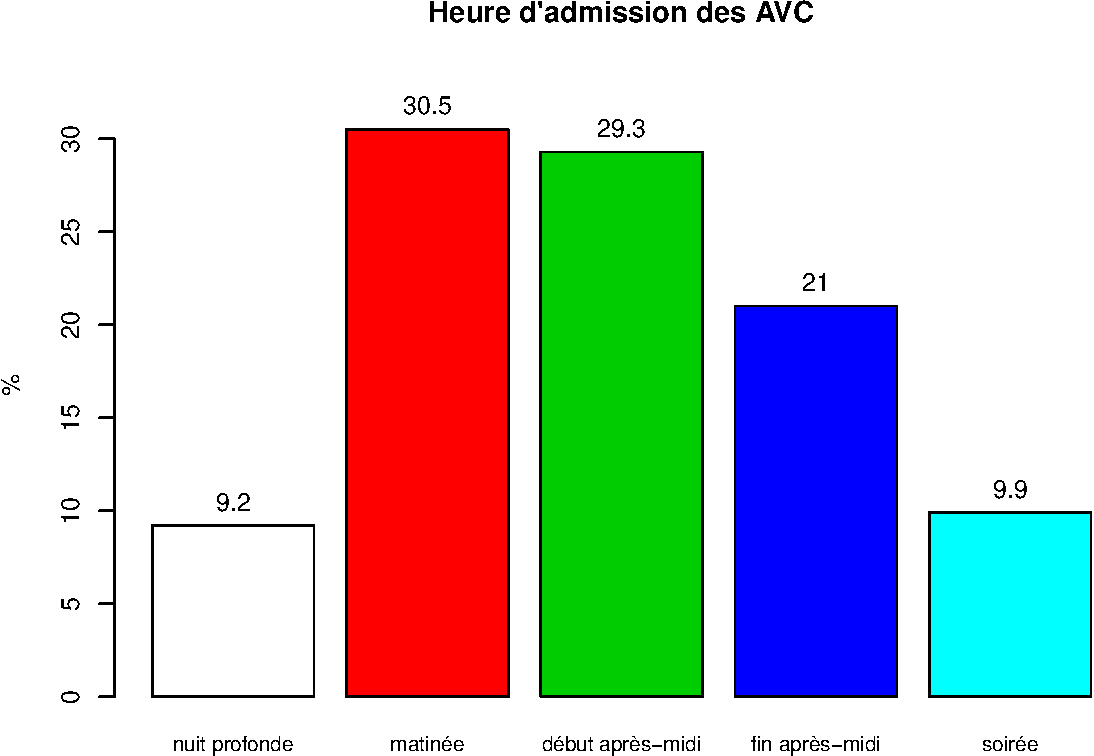
\includegraphics{rapport2014_V4_files/figure-latex/avc_periode-1.pdf}

\begin{itemize}
\item
  \% AVC le matin: 30.5 \%.
\item
  \% AVC en début d'après-midi: 29.3 \%.
\item
  \% AVC en fin d'après-midi: 21 \%.
\item
  \% AVC en soirée: 9.9 \%.
\item
  \% AVC le nuit profonde: 9.2 \%.
\item
  Nombre de passages AVC urgences, déclinaison par département,
  établissement, année N
\end{itemize}

\begin{verbatim}
## 3Fr Alk Ane Col Dia Dts Geb Hag Hus Mul Odi Ros Sav Sel Wis 
##  63  30  NA 741  NA  NA  30 500 580 682  NA  NA  NA 238  85
\end{verbatim}

\begin{itemize}
\item
  \% passages en horaire de PDS

  \begin{longtable}[c]{@{}rlll@{}}
  \toprule\addlinespace
  PDS & S PDS & WE NPD & S
  \\\addlinespace
  \midrule\endhead
  Nombre AVC & 403 & 656 & 1890
  \\\addlinespace
  \% AVC & 14 & 22 & 64
  \\\addlinespace
  \bottomrule
  \end{longtable}
\end{itemize}

PDSS = horaires de PDS en semaine, PDSWE = horaires de PDS le WE, NPDS =
hors horaire de PDS.

\begin{itemize}
\itemsep1pt\parskip0pt\parsep0pt
\item
  nombre d'AVC aux horaires de PDS en semaine: 13.67 \%
\item
  nombre d'AVC aux horaires de PDS de week-end:22.24 \%
\item
  nombre d'AVC en dehors des horaires de PDS:64.09 \%
\end{itemize}

\subsection{Mode d'arrivée aux
urgences}\label{mode-darrivee-aux-urgences}

\begin{itemize}
\itemsep1pt\parskip0pt\parsep0pt
\item
  \% d'arrivées Moyen perso: 21.57\%
\item
  \% d'arrivées SMUR: 1.97\%
\item
  \% d'arrivées VSAV: NA\%
\item
  \% d'arrivées ambulance privée: 39.13\% NB : commentaire possible pour
  expliquer que la somme des 4 pourcentages ci dessus ne fait pas 100 \%
\end{itemize}

\subsection{DIAGNOSTIC PRINCIPAL}\label{diagnostic-principal-1}

\begin{itemize}
\itemsep1pt\parskip0pt\parsep0pt
\item
  Nombre d'AVC ischémique et \%: 1 021 (34.62 \%)
\item
  Nombre d'AIT et \%: 806 (27.33 \%)
\item
  Nombre de codes ``symptomatiques'' (hémiplégie, aphasie, amaurose,
  etc\ldots{}) et \%
\item
  Nombre d'autres hémorragies non traumatiques et \%: 442 (14.99 \%)
\end{itemize}

NB : se référer à l'annexe 4 pour les regroupements.

\subsection{DURÉE}\label{duree-1}

Voir ligne 333

Voir les routines de RPU\_2014/Analyse/Temps\_passage/passage.R et
notamment \textbf{temps de passage}.

\begin{itemize}
\itemsep1pt\parskip0pt\parsep0pt
\item
  Durée de passage (HORS UHCD) année N: moyenne \textbf{249.8} minutes,
  et médiane \textbf{228} minutes.
\item
  \% de passages de moins de 4h 0.92
\end{itemize}

\subsection{MODE DE SORTIE}\label{mode-de-sortie-2}

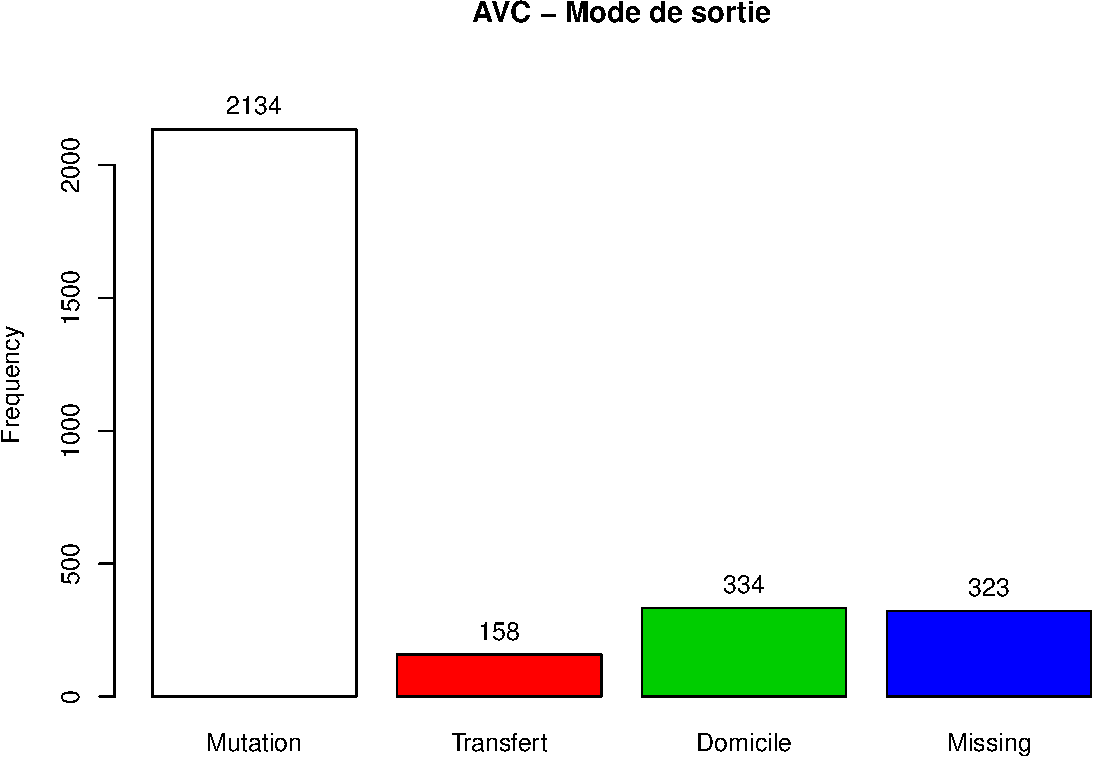
\includegraphics{rapport2014_V4_files/figure-latex/avc_mode_sortie-1.pdf}

\begin{itemize}
\itemsep1pt\parskip0pt\parsep0pt
\item
  \% d'hospitalisation: 87.3 \%
\item
  \% de mutation: 81.3 \%
\item
  \% de transfert: 6 \%
\item
  \% de retour à domicile: 12.7 \%
\end{itemize}

\subsection{Orientation}\label{orientation}

\begin{itemize}
\itemsep1pt\parskip0pt\parsep0pt
\item
  Répartition par orientation en pourcentage, année N
\end{itemize}

\% Table created by stargazer v.5.1 by Marek Hlavac, Harvard University.
E-mail: hlavac at fas.harvard.edu \% Date and time: Ven, jul 31, 2015 -
16:26:10

\begin{table}[!htbp] \centering 
  \caption{Orientation des AVC} 
  \label{orientation} 
\begin{tabular}{@{\extracolsep{5pt}} cccccccccc} 
\\[-1.8ex]\hline 
\hline \\[-1.8ex] 
CHIR & FUGUE & HO & MED & REA & SC & SCAM & SI & UHCD & NA's \\ 
\hline \\[-1.8ex] 
$75$ & $1$ & $1$ & $720$ & $68$ & $46$ & $9$ & $361$ & $919$ & $749$ \\ 
\hline \\[-1.8ex] 
\end{tabular} 
\end{table}

\subsection{Doublons ?}\label{doublons}

\begin{itemize}
\itemsep1pt\parskip0pt\parsep0pt
\item
  Age moyen, année N
\item
  Répartition par classe âge en pourcentage, année N
\item
  Répartition par sexe en pourcentage, année N
\item
  TOP 5 pourcentage par code CIM 10, année N
\item
  Répartition we/semaine en pourcentage, année N
\item
  Répartition par tranche heure en pourcentage, année N
\end{itemize}

\section{ANNEXES}\label{annexes}

\subsection{ANNEXE 1 : Définitions}\label{annexe-1-definitions}

\subsection{ANNEXE 2 : Diagramme de complétude des
RPU}\label{annexe-2-diagramme-de-completude-des-rpu}

\subsection{ANNEXE 3 : Calcul du TARRU}\label{annexe-3-calcul-du-tarru}

\section{Information de session}\label{information-de-session}

\begin{verbatim}
R version 3.1.3 (2015-03-09)
Platform: x86_64-apple-darwin13.4.0 (64-bit)
Running under: OS X 10.10.3 (Yosemite)

locale:
[1] fr_FR.UTF-8/fr_FR.UTF-8/fr_FR.UTF-8/C/fr_FR.UTF-8/fr_FR.UTF-8

attached base packages:
[1] stats     graphics  grDevices utils     datasets  methods   base     

other attached packages:
 [1] openintro_1.4     xtable_1.7-4      stargazer_5.1    
 [4] epicalc_2.15.1.0  nnet_7.3-10       MASS_7.3-42      
 [7] survival_2.38-3   foreign_0.8-65    R.utils_2.1.0    
[10] R.oo_1.19.0       R.methodsS3_1.7.0 xts_0.9-7        
[13] zoo_1.7-12        plotrix_3.5-12    lubridate_1.3.3  
[16] knitr_1.10.5     

loaded via a namespace (and not attached):
 [1] digest_0.6.8    evaluate_0.7    formatR_1.2     grid_3.1.3     
 [5] highr_0.5       htmltools_0.2.6 lattice_0.20-31 magrittr_1.5   
 [9] memoise_0.2.1   plyr_1.8.3      Rcpp_0.11.6     rmarkdown_0.7  
[13] splines_3.1.3   stringi_0.5-5   stringr_1.0.0   tools_3.1.3    
[17] yaml_2.1.13    
\end{verbatim}

\begin{verbatim}

To cite R in publications use:

  R Core Team (2015). R: A language and environment for
  statistical computing. R Foundation for Statistical Computing,
  Vienna, Austria. URL http://www.R-project.org/.

A BibTeX entry for LaTeX users is

  @Manual{,
    title = {R: A Language and Environment for Statistical Computing},
    author = {{R Core Team}},
    organization = {R Foundation for Statistical Computing},
    address = {Vienna, Austria},
    year = {2015},
    url = {http://www.R-project.org/},
  }

We have invested a lot of time and effort in creating R, please
cite it when using it for data analysis. See also
'citation("pkgname")' for citing R packages.
\end{verbatim}

\end{document}
